\documentclass[12pt,a4paper]{report}
\usepackage{amsmath}
\usepackage{amsfonts}
\usepackage{amssymb}
\usepackage{fullpage}
\usepackage[slovak]{babel}
\usepackage[utf8]{inputenc}
\usepackage[T1]{fontenc}
\usepackage{fullpage}
\usepackage{indentfirst}
\usepackage{array}
\usepackage{graphicx}
\DeclareGraphicsExtensions{.png,.jpg}

\begin{document}
\begin{titlepage}
\centering\bfseries
		Fakulta matematiky, fyziky a informatiky\\Univerzita Komenského v Bratislave	
	\vspace*{\stretch{2.0}}

	\fontsize{23}{28}\textbf{Špecifikácia požiadaviek na softvér}\\
	\vspace*{\stretch{0.05}}
	\fontsize{16}{22}\textbf{Predikcia šírenia infekčných ochorení}\\
	\vspace*{\stretch{0.2}}
	\large\textit{Matúš Čongrády\\Tibor Hanesz\\Jonatan Foltyn\\Katarína Šimnová}

	\vspace*{\stretch{2.0}}
\end{titlepage}\bigskip
	\setcounter{tocdepth}{9}
	\tableofcontents
	
\renewcommand{\chaptername}{}	
\chapter[Konceptuálna analýza]{\rmfamily\bfseries
	Konceptuálna analýza}
	
\section[Používateľské rozhranie]{\rmfamily\bfseries
	Používateľské rozhranie}
Táto  časť  bude  venovaná približnému  grafickému  opisu užívateľského  rozhrania. Opisuje aké komponenty sa na akých stránkach budú nachádzať a čo bude ich želaným vstupom.

\subsection[Hlavná stránka]{\rmfamily\bfseries
	Hlavná stránka}

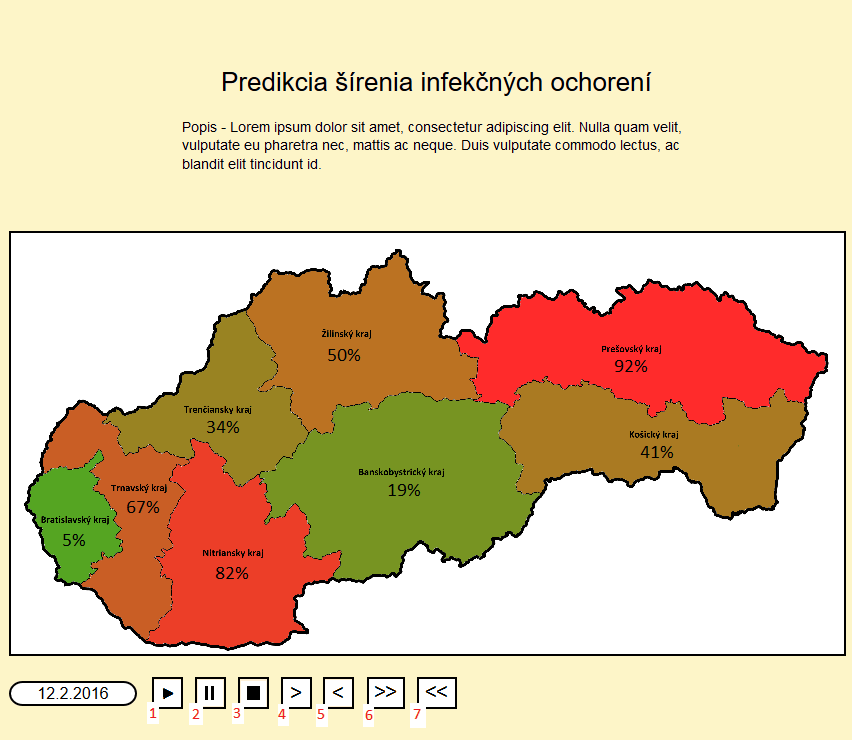
\includegraphics[scale=0.7]{hl_stranka}

\begin{table}[h!]
	\centering
	\begin{tabular}{|>{\centering\arraybackslash}m{3in}|>{\centering\arraybackslash}m{3in}|}
		\hline
		\centering Parameter & Vlastnosti \\ [0ex]
		\hline
		Mapa & Miesto zobrazenia animácie šírenia infekčného ochorenia.\\ [0ex]
		\hline
		Deň &  Oznáčuje deň pre ktorý animacáacia v danom momente zobrazuje štatistiku.\\ [0ex]
		\hline
		1. & Spustenie animácie.\\ [0ex]	
		\hline
		2. & Zastavenie animácie.\\ [0ex]	
		\hline
		3. & Vypnutie animácie.\\ [0ex]	
		\hline
		4. & Prechod o jeden deň vpred.\\ [0ex]	
		\hline
		5. & Prechod o jeden deň vzad.\\ [0ex]	
		\hline
		6. & Zrýchlenie animácie.\\ [0ex]	
		\hline
		7. & Spomalenie animácie.\\ [0ex]	
		\hline

	\end{tabular}
\end{table}

\subsection[Prihlásenie]{\rmfamily\bfseries
	Prihlásenie}

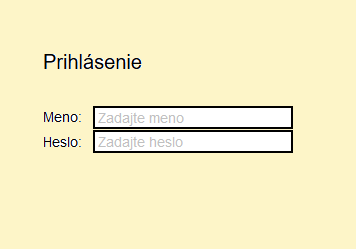
\includegraphics[scale=0.7]{prihlasenie}

\begin{table}[h!]
	\centering
	\begin{tabular}{|>{\centering\arraybackslash}m{3in}|>{\centering\arraybackslash}m{3in}|}
		\hline
		\centering Parameter & Vlastnosti \\ [0ex]
		\hline
		Meno & Užívateľ zadá svoje prihlasovacie meno.\\ [0ex]
		\hline
		Heslo & Užívateľ zadá svoje prihlasovacie heslo. \\ [0ex]
		\hline
	\end{tabular}
\end{table}

\subsection[Administrácia]{\rmfamily\bfseries
	Administrácia}

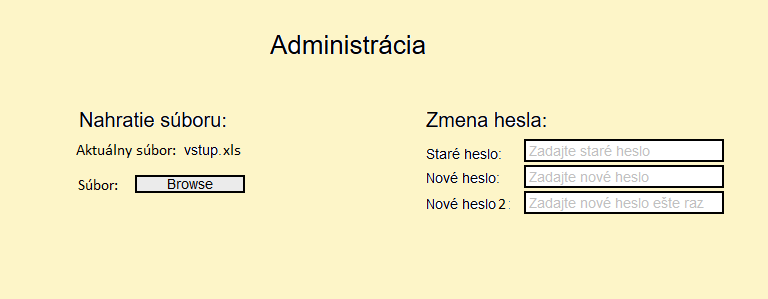
\includegraphics[scale=0.7]{admin}

\begin{table}[h!]
	\centering
	\begin{tabular}{|>{\centering\arraybackslash}m{3in}|>{\centering\arraybackslash}m{3in}|}
		\hline
		\centering Parameter & Vlastnosti \\ [0ex]
		\hline
		Aktuálny súbor & Label zobrazujúci názov súboru aktuálne použitého vstupu.\\ [0ex]
		\hline
		Súbor & Užívateľ  vyberie  validný  XLS súbor obsahujúci maticu. \\ [0ex]
		\hline
		Staré heslo & Užívateľ zadá svoje pôvodné heslo.\\ [0ex]	
		\hline
		Nové heslo & Užívateľ zadá svoje nové heslo. \\ [0ex]		
		\hline
		Nové heslo 2 & Užívateľ zadá svoje nové heslo druhýkrát. \\ [0ex]		
		\hline
	\end{tabular}
\end{table}

\section[Možnosti užívateľa]{\rmfamily\bfseries
	Možnosti užívateľa}

\subsection[Stavový diagram]{\rmfamily\bfseries
	Stavový diagram}

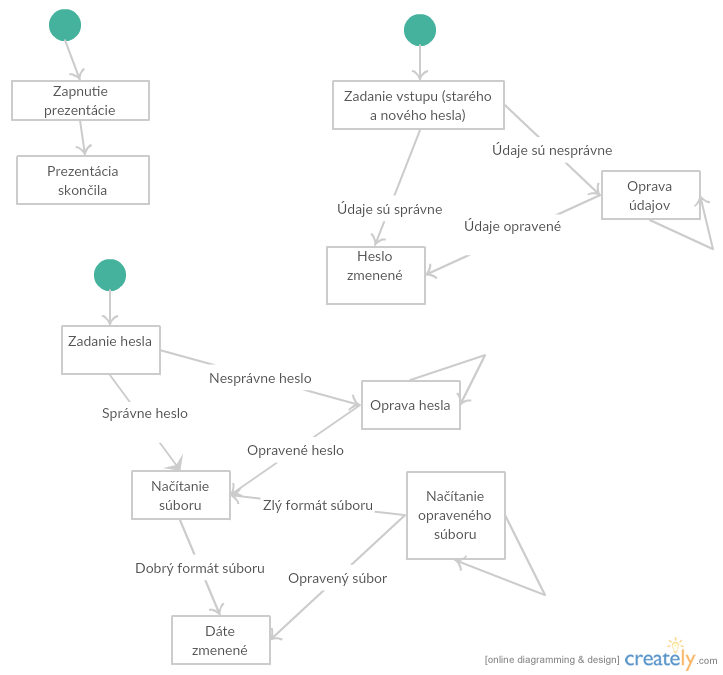
\includegraphics[scale=0.6]{Stavovy_diagram}

\end{document}